% Chapter Template
\chapter{Audio Processing} % Main chapter title

\label{Chapter5} % Change X to a consecutive number; for referencing this chapter elsewhere, use \ref{ChapterX}
Before we feed the audio clip to our machine learning model, it is crucial to pre-process the signal as to achieve higher accuracy
and avoid further deterioration.
The choice and implementation of noise filter will then be explained in \textbf{LINK TO SECTION 1}. We then feed the filtered output 
to a pitch detection algorithm (PDA) \textbf{lINK TO SECTION 2} and then a key detection algorithm (KDA) \textbf{LINK TO SECTION 3}
Figure \textbf{UPDATE!} shows the flowchart of the audio processing part of our project.

% \begin{figure}
% \tikzset{
% every edge/.style = {draw=cyan, line width=2mm, shorten >=1pt, shorten <=1pt,
%                      -{Triangle[scale=0.6]}},
% N/.style args = {#1/#2}{fill=#1, text width=#2, 
%                         font=\scriptsize, align=center},
%    N/.default = cyan/7em,
% }
% \newcommand\tn[1]{\textbf{\small #1}}
%     \begin{tikzpicture}[node distance=8mm]
% \node (n1) [N]  {\tn{User sings into our app}\\ 
%                  (Obtain input audio signal)}; 
% \node (n2) [N=cyan/8em, right=of n1] 
%                 {\tn{Trim silence at the start/end of audio clip};
% \node (n3) [N, right=of n2] 
%                 {\tn{Implement noise filter}};
% \node (n4) [N, below=of n3]
%                 {\tn{Spectral reduction}};
% \node (n5) [N, right=of n4]
%                 {\tn{Low-pass filter}};
% \node (n6) [N, right=of n3] 
%                 {\tn{Implement PDA}};
% \node (n7) [N, right=of n6] 
%                 {\tn{Implement KDA}};
% \node (n8) [N=red!30/8em, below=of n7]
%                 {\tn{Pass the output to Ed's ML model}\\
% 				(Notes and keys)};

% \draw   (n1) edge (n2)
%         (n2) edge (n3)
%         (n3) edge (n4)
% 		(n4) edge (n5)
%         (n3) edge (n6)
%         (n6) edge (n7)
% 		(n7) edge (n8));
%     \end{tikzpicture}
% \end{figure}
%----------------------------------------------------------------------------------------
%	SECTION 0
%----------------------------------------------------------------------------------------
\section{Assumptions}
Before we delineate the approach to audio processing, there are some assumptions that our model
is built on:
\begin{itemize}
	\item \textbf{Assumption 1:} Users' audio input device does not contain active noise cancelling functions.
\end{itemize}

These assumptions will be referred to later on in the section.
%----------------------------------------------------------------------------------------
%	SECTION 1
%----------------------------------------------------------------------------------------

\section{Noise Filter}
Noise filtering is essential as it reducess or eliminates the noise present in the input signal.
A conventional method to quantify noise is to use signal-to-noise ratio (SNR), which is often 
represented in decibels.
\[SNR=10*log_10((P_{signal})/(P_{noise}))\]
As its name suggests, SNR is the power ratio between desired signal and undesired noise. Effectively,
we would like to use noise filters to achieve a higher SNR.\\ 
There is a few sources of noise when an user record himself with a microphone.
Firstly, there exists self-noise, which is the instrument noise produced by the microphone itself.
Noise may be induced or created when the signal passes through electronic componenets like transistors 
and printed circuit boards.\cite{selfnoise} 
The second source, ambient noise, contributes to a large portion of noise present in a recording.
Room reflections, extraneous noise, electromagnetic interference and mechanical noise are some causes 
to the existence of ambient noise. 
%-----------------------------------
%	SUBSECTION 1
%-----------------------------------
\subsection{Possible Models}
Most of the noise filters work in the frequency and spectral domain, here we are going to inspect and
compare 3 noise reduction mechanisms.

\begin{enumerate}
	\item Low-pass filter (LPF)\\
	LPF passes signals with \(f<f_{c}\), where \(f_{c}\) is the cut-off frequency, and attenuates
	signals with \(f>fc\). 
	\[H(f) = rect(f/(2*B))\]
	\[h(t))= \mathfrak{F}^-1{H(f)} = \int_{-B}^{B} e^(2(\pi)ift)\,df = 2Bsinc(2Bt)\]
	In order to implement an LPF, we have to transform signal from time domain to 
	frequency domain using fourier transform. An ideal LPF would completely remove frequencies that are
	higher than \(f_{c}\) and is a non-ca)sual linear time-invariant system. The impulse
	response of an LPF is a sinc function that extends to [$\infty$,-$\infty$]. This is why it is impossible to 
	realize an ideal LPF since that will take infinite time and memory.\\
	LPF avoids aliasing since it removes the high-frequency content but not the desired signal

	\item Wavelet transform\\
	Wavelet transform creates a representation of the signal in both time and frequency domain so localized 
	information of the signal can be efficiently accessed. It is often compared with fourier transform (FT), which
	has the below limitations: 
	\begin{enumerate}
		\item For windowed FT, if the feature is larger or shorter than the window, it cannot be captured completely.
		\item Time resolution for high frequencies is the same for low frequencies. As frequency increases, rate of 
		change of the signal increases, and high frequency signals contain more information in a window than that of 
		low frequency, thus we need a higher time resolution for that.
	\end{enumerate}
	Wavelet transform analyzes a signal by its different frequency components at multiple resolution so features that are 
	undiscovered at one resolution may be obvious at another. There are mainly 2 types of wavelet transforms, namely 
	continuous wavelet transform (CWT) and discrete wavelet transform (DWT) and here are the mathematical representations
	for the two transforms:
	CWT finds how alike a wavelet is in a signal, given the above 2 properties that the wavelet has. \cite{wavelet}
	This can be found by convolving the mother wavelet with our signal.

	\begin{equation*} 
		\text{CWT}(\mathrm{a},\mathrm{b}; \mathrm{x}(\mathrm{t}),\psi(\mathrm{t}))=\int_{-\infty}^{\infty}[\mathrm{x}(\mathrm{t})\frac{1}{\mathrm{a}}-\psi^{*}(\frac{\mathrm{t}-\mathrm{b}}{\mathrm{a}})]\text{dt}
	\end{equation*}\cite{wavelet_denoise}

	where $x(t)$ is the original signal, $\psi(t)$ is the mother wavelet, $a$ is a dilation parameter and $b$ is a translation parameter.
	Dilation factor represents how dispersed the wavelet is (similar to scaling) while translation factor tells us where the wavelet is
	positioned in time (similar to shifting). 
	
	\begin{figure}
		\centering
		\begin{subfigure}{.3\textwidth}
		  \centering
		  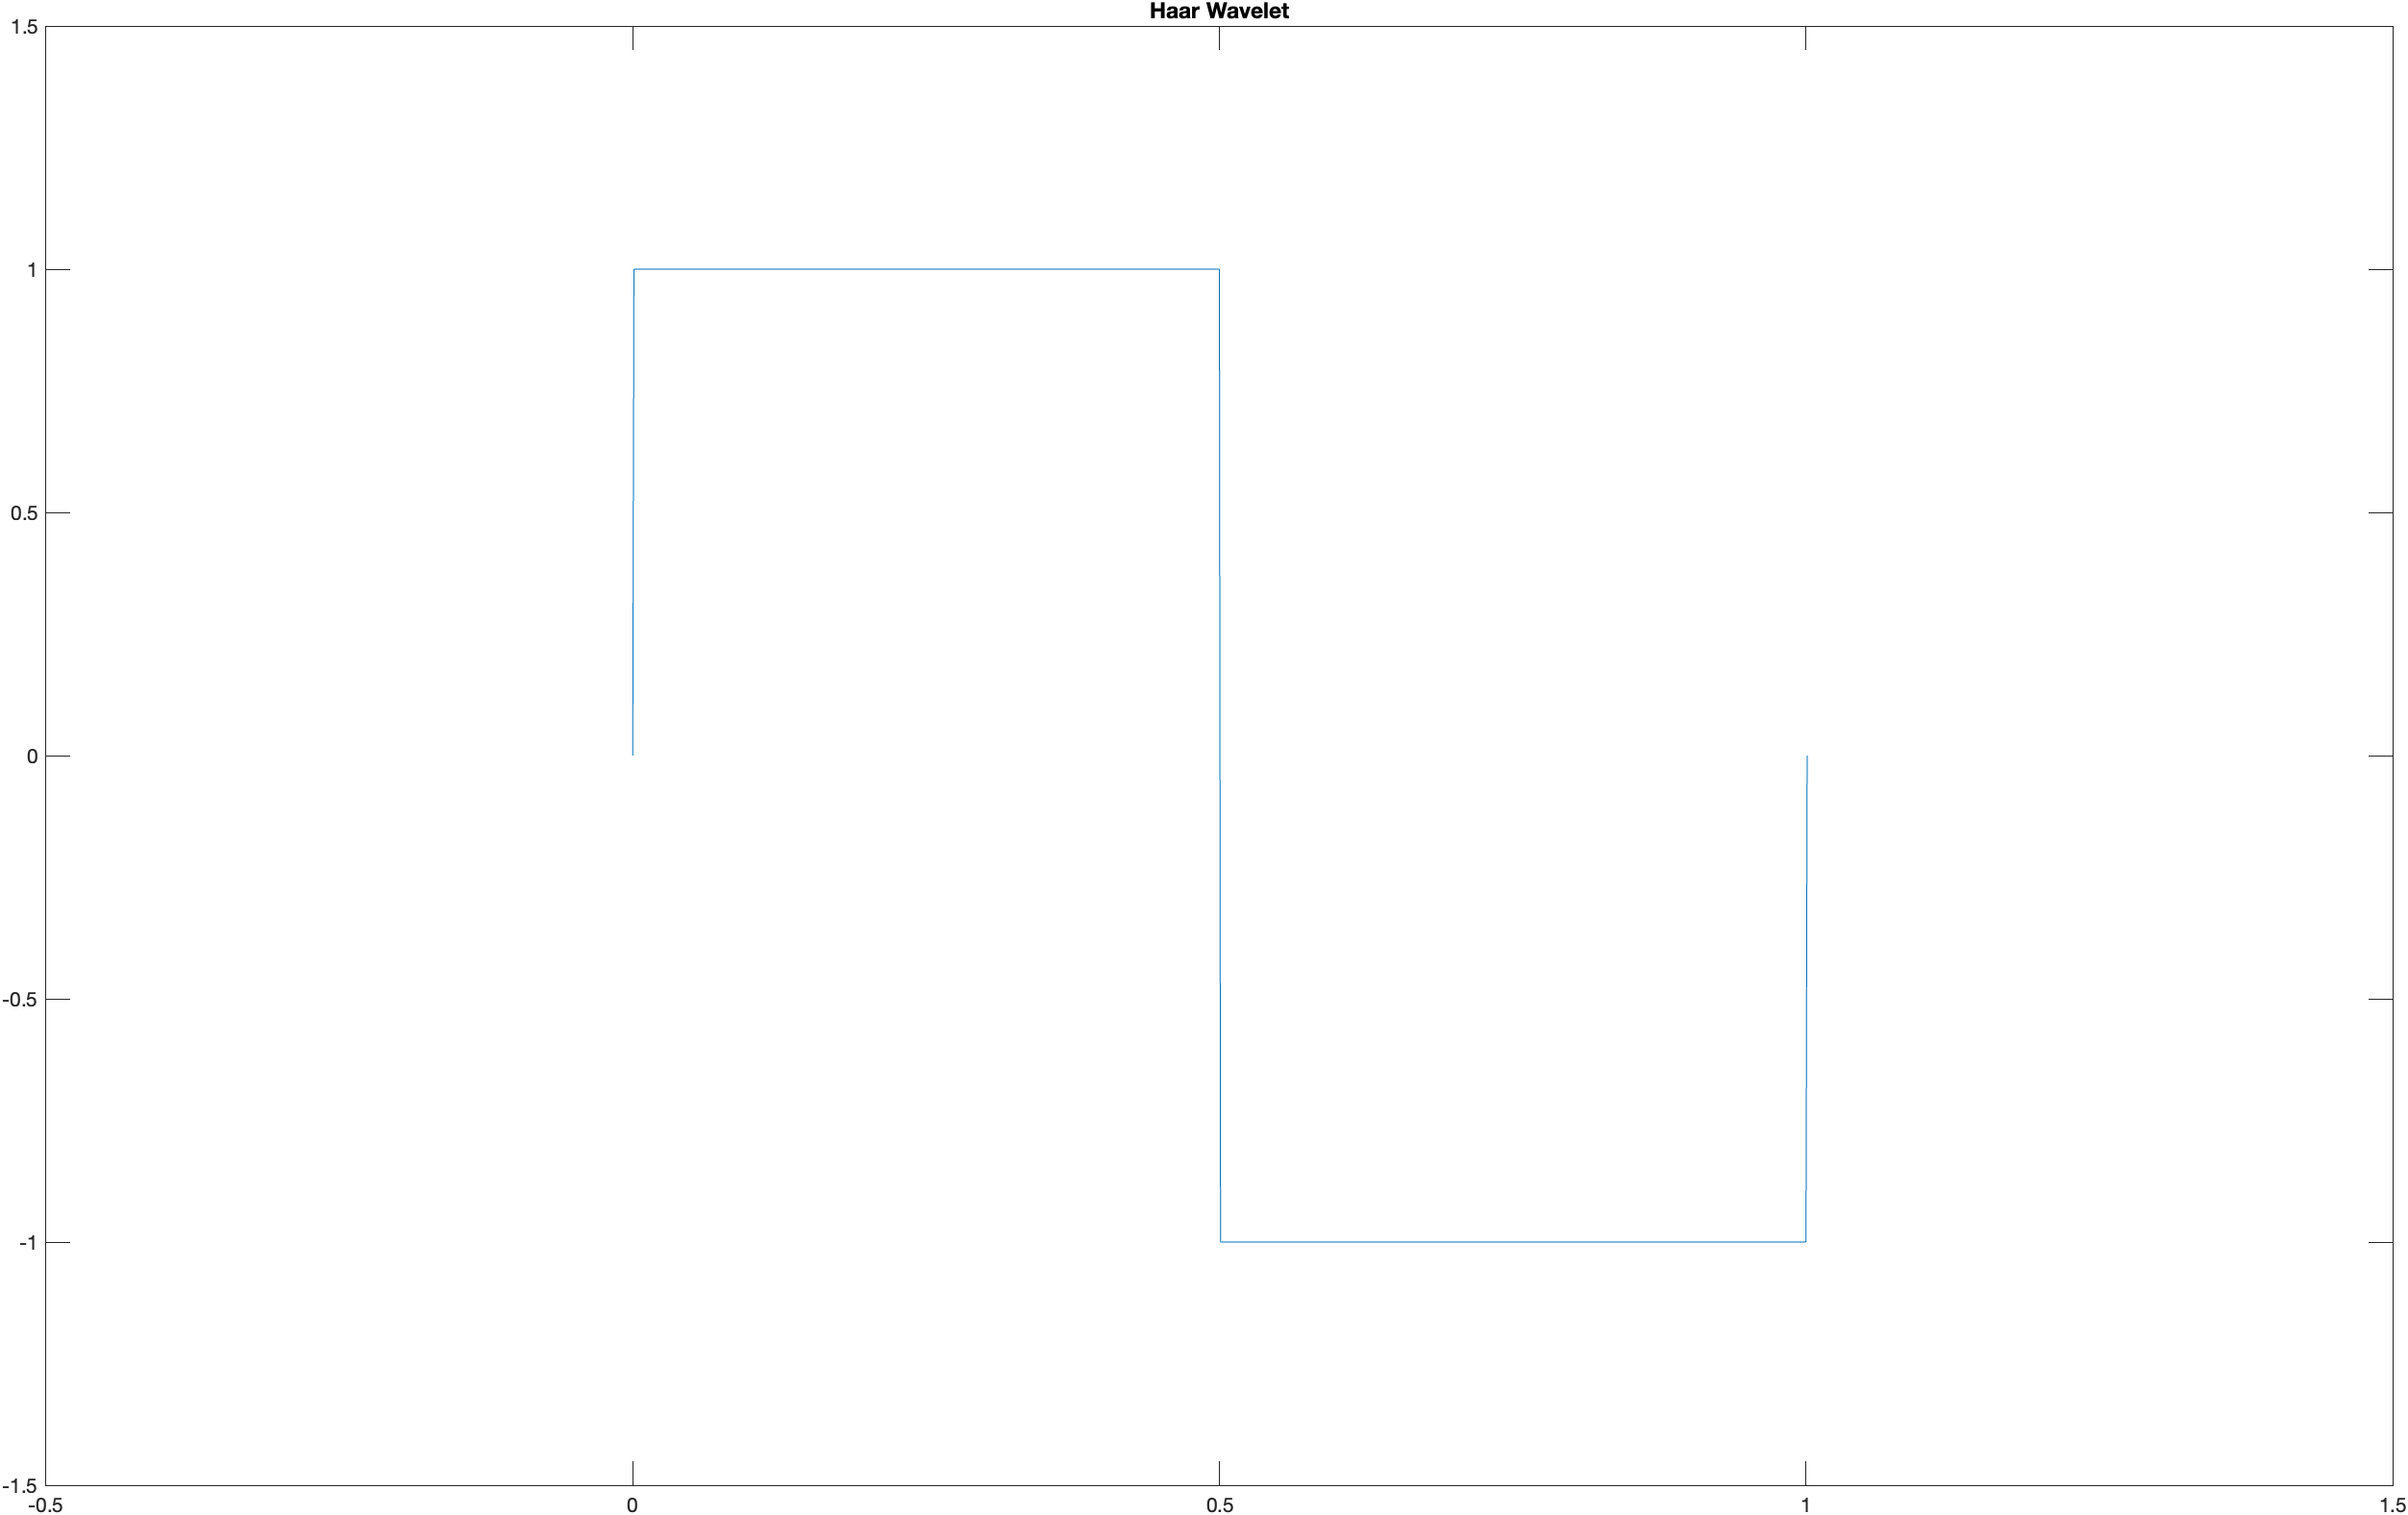
\includegraphics[width=\linewidth]{haar.png}
		  \caption{Haar wavelet}
		  \label{Haar}
		\end{subfigure}%
		\begin{subfigure}{.3\textwidth}
			\centering
			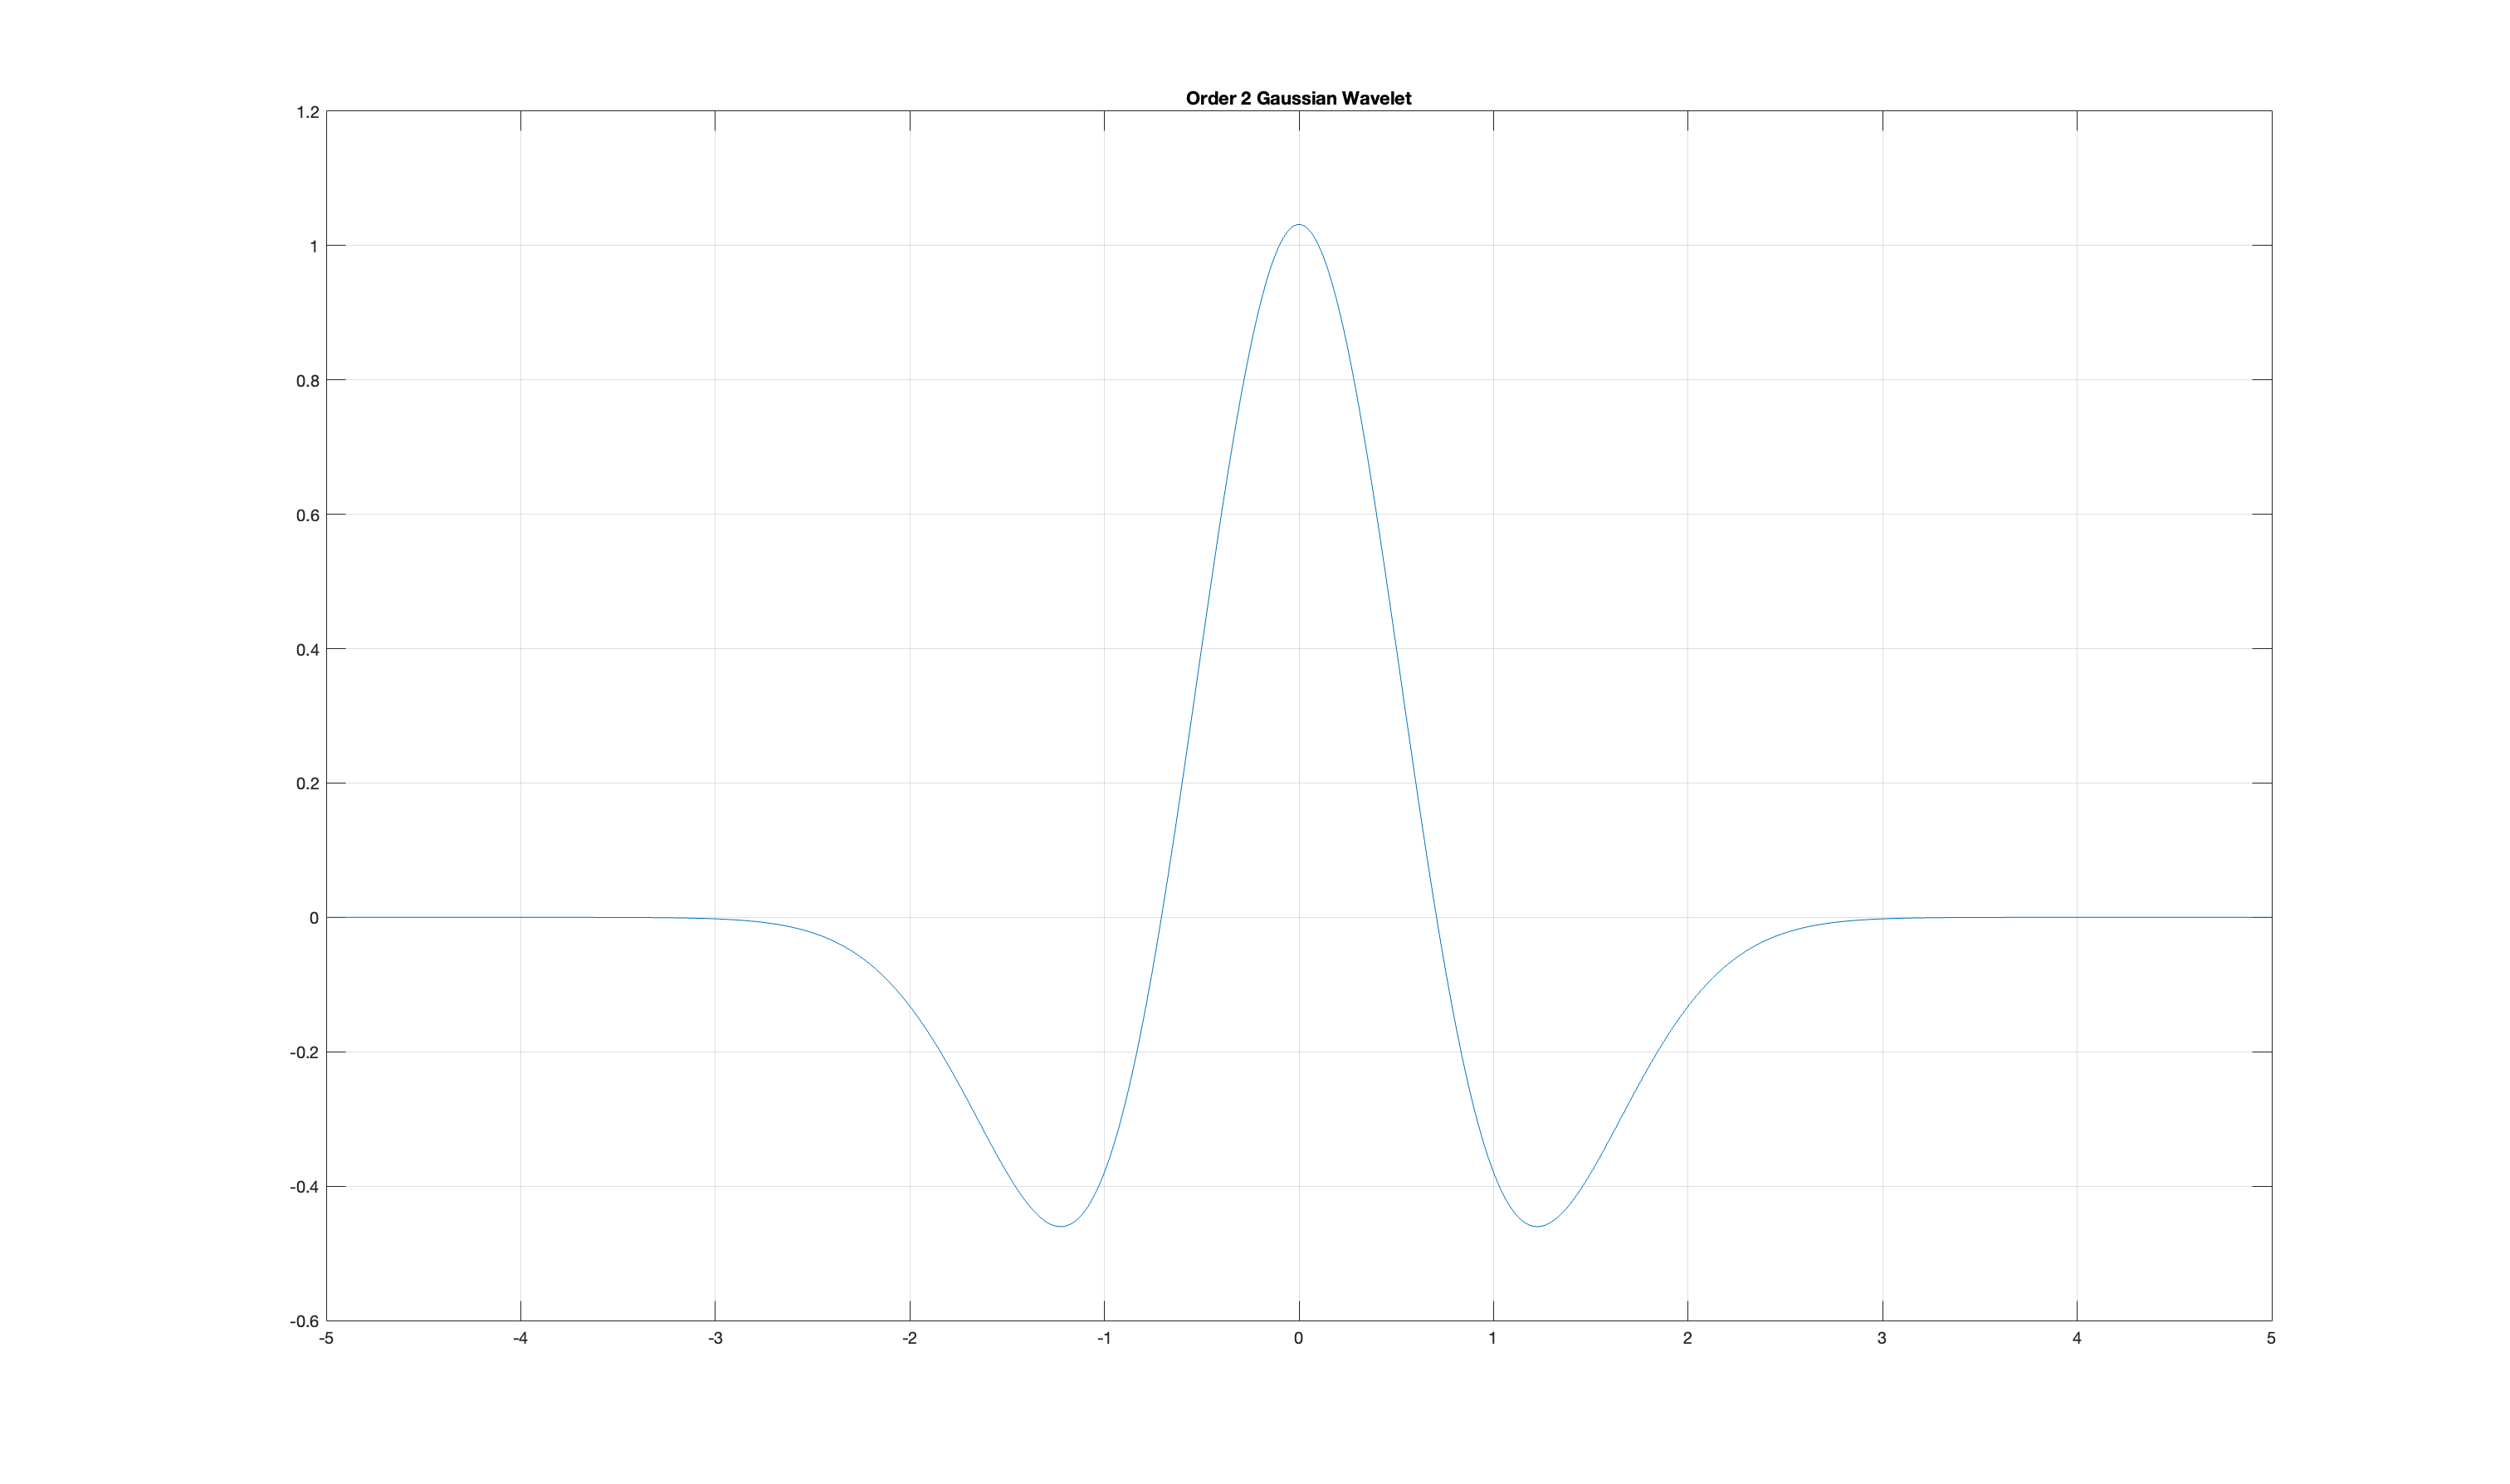
\includegraphics[width=\linewidth]{order2gaussian.png}
			\caption{Gaussian wavelet of order 1}
			\label{order1}
		  \end{subfigure}%
		\begin{subfigure}{.3\textwidth}
		  \centering
		  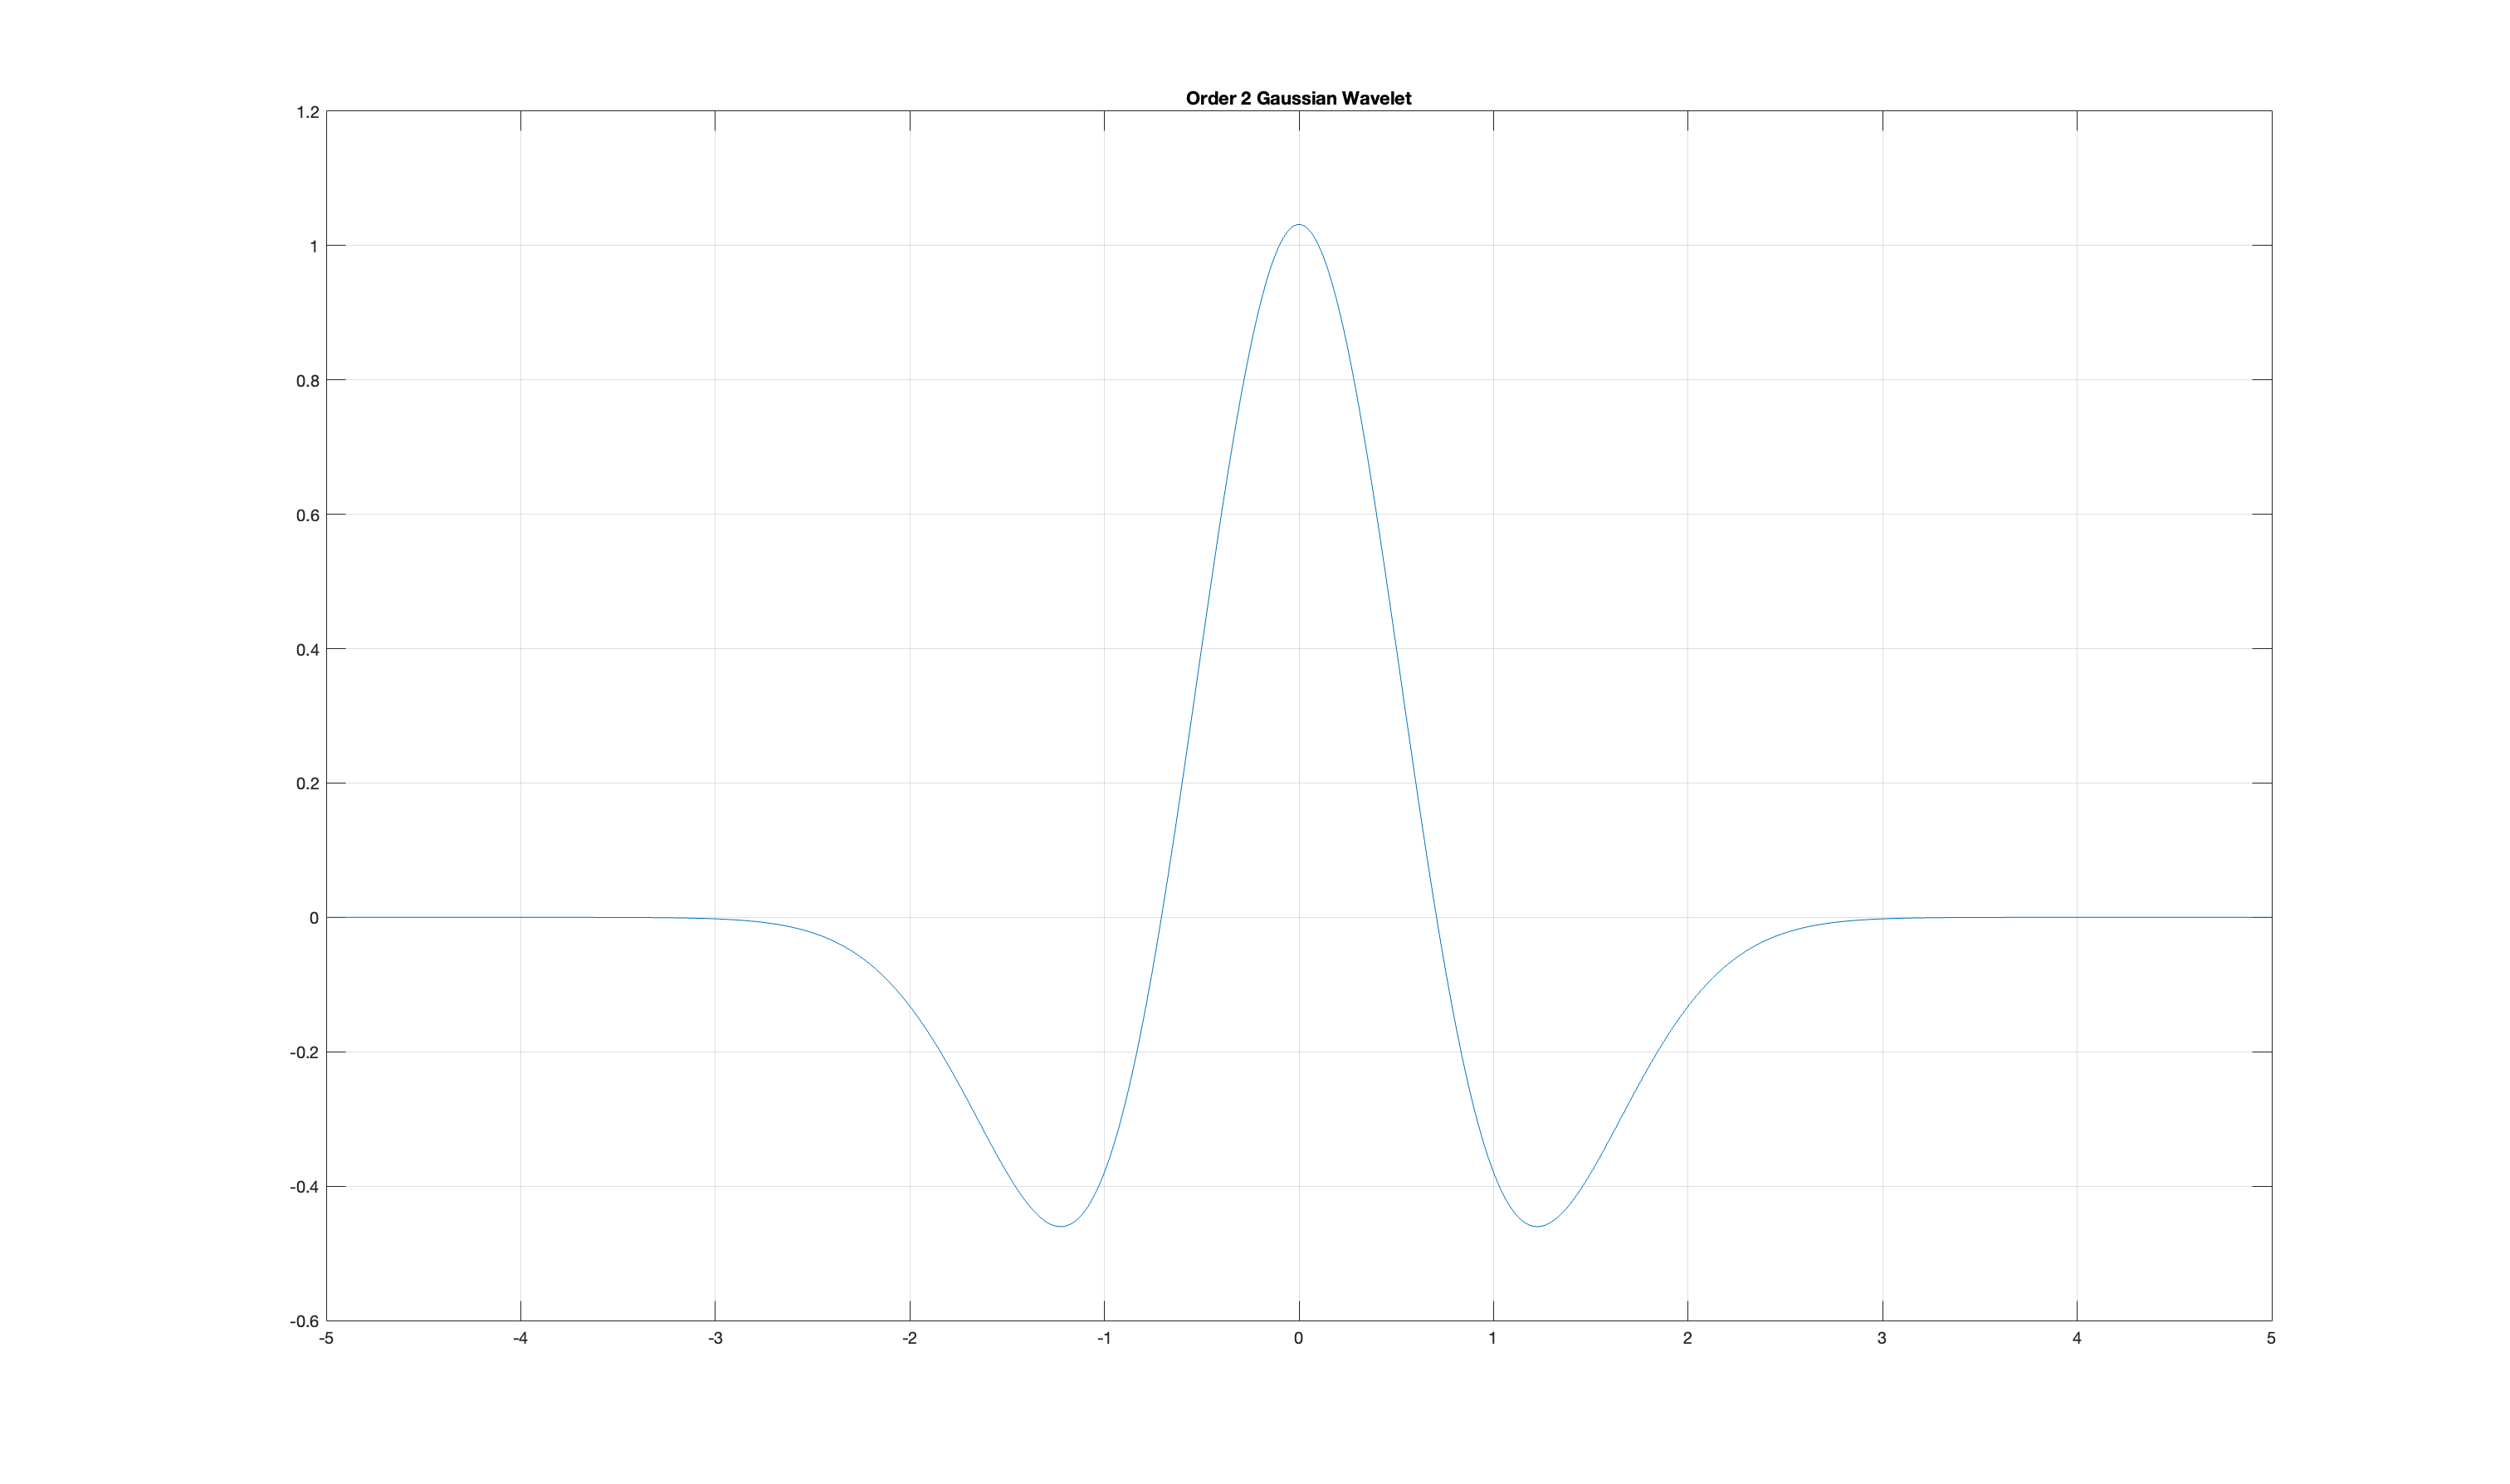
\includegraphics[width=\linewidth]{order2gaussian.png}
		  \caption{Ricker wavelet - Gaussian wavelet of order 2}
		  \label{Ricker}
		\end{subfigure}%
		\caption{Examples of wavelets}
		\label{fig:test}
	\end{figure}
	
	\begin{align*} &\text{DWT}\ [\mathrm{n},\mathrm{a}^{\mathrm{j}}]=\sum_{\mathrm{m}=0}^{\mathrm{N}-1}\mathrm{x}[\mathrm{m}].{\psi_{\mathrm{j}}}^{*}[\mathrm{m}-\mathrm{n}],\\ &\psi_{\mathrm{j}}[\mathrm{n}]=\frac{1}{\sqrt{\mathrm{a}^{\mathrm{f}}}}\psi\left(\frac{\mathrm{n}}{\mathrm{a}^{\mathrm{f}}}\right) \tag{2} \end{align*}
	where $n$ is delay parameter, $N$ is the length of signal, $\psi$ is the discretized mother wavelet. \cite{wavelet_denoise}

	We will focus on DWT since computation is done on discrete wavelets so it requires less computational resources.
	% Usually for stationary signals, we use conventional frequency-based filters, but for non-stationary ones, we can 
	% use wavelet transform, in particular continuous wavelet transform (CWT) which gives better time-scale information
	% compared to short-time fourier transform (STFT). 
 
	% Wavelet transform analyses a signal into different frequencies at different resolution (multiresolution analysis). 
	
% 	Wavelets are adjustable and adaptable. Because there is not just one wavelet, they can be designed to fit 
% 	individual applications. They are ideal for adaptive systems that adjust themselves to suit the signal.
% Disadvantages of DWT:
% 	Sensitive to shifting
% 	Poor directionality
% 	Lack of phase information
% 	Hard to choose an appropriate mother wavelet and number of decomposition levels

%more on wavelet denoise: https://citeseerx.ist.psu.edu/viewdoc/download?doi=10.1.1.206.5126&rep=rep1&type=pd
	\item Spectral reduction\\
Suppose noise is additive, and we can represent our noisy audio 
\begin{equation} \label{eq:1}
\y(n) = x(n) + d(n), for 0 <= n <= N-1 
\end{equation}
where $x(n)$ is our original signal (signal we wish to recover), $d(n)$ is the noise, $n$ is the discrete time index,
$N$ is the number of samples. 
Assuming $d(n)$ and $x(n)$ have no correlation, and we perform a short-time fourier transform on equation \textbf{CHANGE!!!1}:
\[Y(\omega,k)= X(\omega,k) + D(\omega,k)\]
where $k$ is the frame number, which can be dropped if we assume the signal is segmented. Each segment will be of
length $N$. We then have the desired signal in frequency domain:
\[X(\omega) = Y(\omega) - N(\omega)\]
Since the statistics of the noise is unknown, we try to find an estimate of noise spectrum by calculating the time-averaged
noise spectrum using parts of the recording that only contain ambient noise. \cite{reductionmanual}
\[\hat{N(\omega)} = \textbf{E}[|N(\omega)|] = (1/N)\sum_{i=0}^{N-1}|N_i(\omega)|\]
We then get the estimated signal spectrum
\[\hat{X(\omega)} = Y(\omega) - \hat{N(\omega)}\]

\end{enumerate}
%-----------------------------------
%	SUBSECTION 2
%-----------------------------------

\subsection{Choice of model and implementation}
After trying to implement all 3 methods, a major difficulty encountered is that it is hard to set the parameters to 
implement for LPF and wavelet transform. For example, since $f_c$ depends on the pitch range of the user and the melody he/ she
is inputting, finding an adequate $f_c$ that separates desired frequencies from undesired ones is hard.
As for wavelet transform, finding an adequate mother wavelet is a difficult task.\\
Although wavelet transform works better for real-life non-stationary signals compared to conventional frequency-based filters, if we
do not feed a suitable mother wavelet, the performance is unsatisfactory, the model cannot distinguish between desired and undesired 
signals and will decrease $P_signal$ at the same time, which is unfavourable when it comes to improving the SNR.\\
Spectral reduction works the best in removing the ambient noise. As for wavelet transform, it is extremely sensitive to



%-----------------------------------
%	SUBSECTION 3
%-----------------------------------

\subsection{Improvements}
The only problem with spectral reduction is that it does not handle extreme responses nicely.


LPF: Cutoff frequency selection: depending on the gender and age, chebyshev? elliptical?
\begin{table}[]
	\begin{tabular}{lll}
																				 & Male   & Female  \\
	Pitch range (Hz)                                                             & 60-180 & 160-300 \\
	\begin{tabular}[c]{@{}l@{}}Praat pitch parameters \\ range (Hz)\end{tabular} & 50-300 & 100-600
	\end{tabular}
\end{table}
%----------------------------------------------------------------------------------------
%	SECTION 2
%----------------------------------------------------------------------------------------

\section{Pitch Detection Algorithm (PDA)}


%-----------------------------------
%	SUBSECTION 1
%-----------------------------------
\subsection{Possible Models}

%-----------------------------------
%	SUBSECTION 2
%-----------------------------------

\subsection{Implementation}

%-----------------------------------
%	SUBSECTION 3
%-----------------------------------

\subsection{Improvements}
(find an algorithm to take in users’ singing frequency to improve accuracy of the model ( perhaps adjust the likelihood of the crepe model?) ( look into automl)

%----------------------------------------------------------------------------------------
%	SECTION 3
%----------------------------------------------------------------------------------------
\section{Key Detection Algorithm (KDA)}

%-----------------------------------
%	SUBSECTION 1
%-----------------------------------
\subsection{Possible Models}

%-----------------------------------
%	SUBSECTION 2
%-----------------------------------

\subsection{Implementation}
